\chapter{Study Two: Hyperdeixis in Advertisements}
\label{studytwo:hyperdeixisinadvertisements}

How do we understand interaction with objects on the Internet? This study considers the role of reference in hyperlinked advertisements. Intentionally misleading or not, ``opt-out'' mechanisms for behavioral advertisements are not intuitive. I believe the cause for confusion is intimately aligned with how we process and understand linguistic signs.

\section{Motivation}
\label{motivation}

In 2009, under pressure from the FTC, industry advertisers formed an alliance called the Digital Advertising Alliance (DAA). The purpose was to establish self-regulatory principles for online behavioral advertising  \citep{AAAA:2009uc}.  These principles advocate transparency for:

\begin{sloppier}
\begin{quote}
[...] clearly disclosing and informing consumers about data collation and user practices with online behavioral advertising [...] Compliance with the Principle will result in new links and disclosures on the web page or advertisement where online behavioral advertising occurs. \citep[p. 2]{AAAA:2009uc}
\end{quote}
\end{sloppier}
Further: 
\begin{quote}
Links to consumer notices will be clear, prominent, and conveniently located... Such enhanced notice will be provided at the time of such collection and use, through common wording and a link/icon that consumers will come to recognize... One option for providing this... is for an entity to attach a uniform link/icon and wording to each advertisement that it serves. Click this link/icon will provide a disclosure from the entity in the form of an expanded text scroll, a disclosure window, or a separate page.  \citep[p. 5]{AAAA:2009uc}
\end{quote}
\begin{sloppier}
This section considers whether DAA self-regulation has designed an effective means for "enhanced notice". 
\end{sloppier}


\subsection{Advertiser Self-Regulation and AdChoices}
\label{advertiserself-regulationandadchoices}

DAA self-regulation has come under repeated fire. The implementation of enhanced notice is the AdChoices icon  (\autoref{adchoices}).  \citet*{Komanduri:2012wo}  examined DAA principles and came up with a list of ten requirements appropriate for compliance checks. Included was a check of whether participating advertisers complied with enhanced notice. One problem is that it is nearly impossible to tell whether a particular ad is behavioral or not. However, they report that according to industry estimates of the time, about 80\% of advertisements encountered are behavioral. Based on this statistic,  \citet{Komanduri:2012wo}  found serious compliance problem including infrequent compliance with ``enhanced notice''.


\begin{figure}
\centerline{

\includegraphics[scale=.5]{chapter6.tex/adchoices}
}
\caption{AdChoices Icon}
\label{adchoices}
\end{figure}


Separately,  \cite{J:2011wm}  manually inspected pages from 449 domestic websites from the Alexa list of top 500 U.S. websites for third-party ads. Only 11.3\% included an AdChoices icon in or around the ad.

Mayer also showed \autoref{original-adchoices} and \autoref{final-adchoices} on his blog at the Center for Internet and Society at Stanford Law School: \cite{J:2011wm}:

\begin{figure}
\centerline{
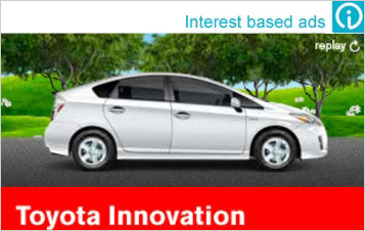
\includegraphics[scale=.75]{chapter6.tex/adchoices_original}
}
\caption{Original AdChoices Design}
\label{original-adchoices}
\end{figure}

\begin{figure}
\centerline{
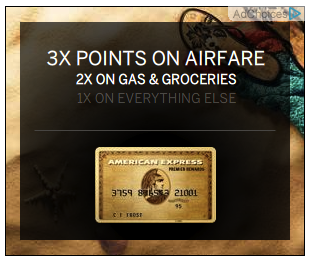
\includegraphics[scale=.5]{chapter6.tex/adchoices_icon_text}
}
\caption{Final AdChoices Design}
\label{final-adchoices}
\end{figure}


Note the differences. According to current DAA Creative Guidelines  \citep{Anonymous:2011ur},  icon only size with container is specified at 19x15 pixels with a rounded left corner radius and 70\% opacity. When embedded in an image, it should be in the upper right corner and there should be no space between it and the ad corner.

\subsection{Effectiveness of the AdChoices Icon}
\label{effectivenessoftheadchoicesicon}

In October of 2012, Evidon served about two billion AdChoices privacy notices daily  \citep{Otlacan:0FDP0X6N}.  This includes delivery across 40 countries and 38 languages. Earlier in 2011, Evidon reported 500,000 ``opt-outs'' as a result of presenting over 50 billion ads  \citep{Dunaway:dVJ7JFhh}.  However,\\

\begin{quote}
[...] those are not "user opt outs" but "company opt outs." For example, if a browser hits an advertiser's opt-out page on Evidon that has 10 ad tech companies listed total, if all are opted out, that counts as 10 opt-outs, even though it's just one browser. \citep{Dunaway:dVJ7JFhh}
\end{quote} 

Disregarding this,  \citet{Dunaway:dVJ7JFhh}  reports the rate of ``opt-out'' at 0.0046\% and  \citet{Logic:2011wn}  reports 0.0035\%.

 \citet{AdChoicesOurExpe:2012ux}  further reports from the period of January 2012 to mid-May 2012, the average daily activity of icon activity was 0.009\% (clicks\slash impression). Of these, 0.003\% were users who had set ``opt-out'' cookies in their browsers.

 \citet{Logic:2011wn}  notes that ``engagement'' in opt-out campaign is influenced by the prominence of the icon --- a white icon container on a black ad --- results in the highest click rates. They also note that ``transparency doesn't foster opt-out''. 1 in 700,000 people who see the icon actually opt-out (about 0.0001\%). Furthermore, they calculate that about 1 in 5 people who make it to the opt-out page actually opt-out. 

It's important to note that that, though AdChoices was introduced in 2010, its rollout to comply with European law was compliancy by 30 June, 2012  \citep{Anonymous:iPLCQu77}. 

\subsection{AdChoices and Confusion}
\label{adchoicesandconfusion}

In a study conducted by  \citet{Ur:2012ws},  48 participants were asked about their familiarity with the DAA advertising icon and older ``Power I'' icon. First, they were presented enlarged icons and tag lines with context. 41 responded they had never seen the icons. Later, presented in context next to advertisements, 25 participants still stated then had never before seen the icons while 8 more were unsure. Only 5 participants thought the icon was intended to provide information about OBA.

This report highlights many usability issues surrounding OBA, to include notice and choice mechanisms. However, they did not address the cause of why AdChoices appears so ineffective.

\subsection{What Makes a Good Ad Design?}
\label{whatmakesagoodaddesign}


\begin{sloppier}
While there is controversy about the effectiveness of "enhanced notice", the advertising industry is actually very good at design. In an online Banner Ad Design Web clinic \citep{BannerAdDesign:2011tg}, Flint McGlaughlin describes three key objectives that banner ads must accomplish in order to drive "maximum conversion".
\end{sloppier}
\begin{enumerate}
\item \textbf{Attract interest.} McGlaughlin gives examples from A/B market tests manipulating size, shape, color, motion, and position toward ad effectiveness.
\item \textbf{Generate interest.} In this, Mclaughlin and others (for example, posts concerning banner ad effectiveness on \url{http://retargeter.com}) focus on the need to understand where targeted consumers might be in the buying process. This principle speaks primarily to tailoring the message to an intended audience.
\item \textbf{"Ask for the Click."} Finally, McLaughlin emphasizes the need for a "call for action". While Internet users implicitly understand that ads are representative of the target site to which they are linked, by placing the image of a button in an ad, McGlaughlin stresses that clarity of the message is increased.
\end{enumerate}


In  \autoref{askforclick} from \cite{BannerAdDesign:2011tg}  and associated audio transcript below, \emph{it is clear to see that while advertisers believe that, despite an understanding that ads convey an implicit message to click, conveying this explicitly is vital}.


\begin{figure}
\centerline{
  
\includegraphics[scale=.25]{chapter6.tex/banner}
  }
\caption{Example "Ask for the Click" \citep{BannerAdDesign:2011tg}}
\label{askforclick}
\end{figure}
\begin{quotation}
Not this, here is an ad [left]. It is animated. They have got motion. Never mind the ugly color. Never mind that it screams the entire time you are looking. Never mind that you have to watch it for a long time before you get the message. Just consider the fact that even once you have watched the whole message, you don't know what to do.

To this, now this ad on the right shows...clearly, we could optimize this way better, but let's just look at this to learn from it. I see a picture of what I am getting, and because it is in a set of hands, I can actually get a sense of the size, and I can imagine it. Never promise a download or any other incentive that you don't help the audience visualize or imagine. Secondly, in the cover and in the key content of the cover, there is appeal already built for somebody in this space, and it is a well-known brand, and then, here it says, get everything you need to know about antiques right in the palm of your hand.

That is also quite helpful in understanding what the offer is, but these people have identified that at this stage, the person may not be ready to buy the book. They may want more info. That is the difference between saying a button 'Buy It Now'. You know, 'Get Your Copy' and instead 'Learn More'. \citep{BannerAdDesign:2011tg}
\end{quotation}


Finally, by regarding current ad images on  \url{http://moat.com} (\autoref{moat}),  it is evident that iconic buttons in image-based ads are highly desirable. This is the case, whether these are flash-based ads (buttons are functional) or simple image-based ads (buttons merely iconic).


\begin{figure}
\centerline{
  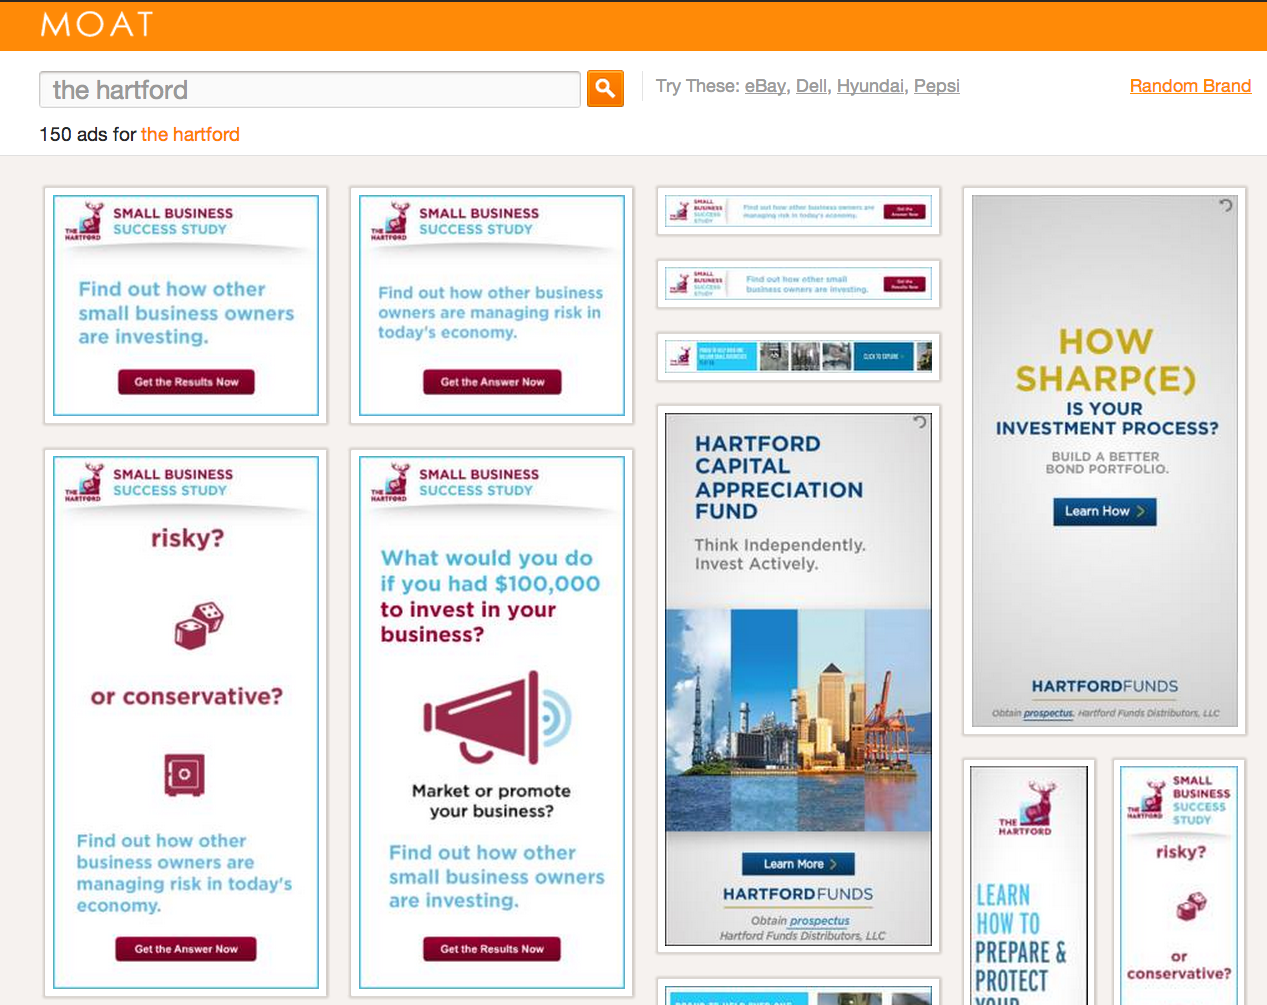
\includegraphics[scale=.25]{chapter6.tex/moat}
  }
\caption{Screen Capture from \url{http://moat.com}}
\label{moat}
\end{figure}


\section{Related Research}
\label{relatedresearch}

Advertising is an intensely competitive business, so it is not surprising that specific details about the effectiveness of the AdChoices icon are difficult to ascertain. Research presented below is directed toward iconicity and indexicality of ads and their parts. This relates to the notion of a ``call-to-action''.

\subsection{Salience}
\label{salience}

Foundational to the representational use of an icon in an ad is whether or not it is perceived in a composite image. Low-level visual properties have a potentially large effect on users.  \citet*{Hoffman:1997vx}  find that the saliency of a part depends on at least three factors: size relative to the whole object, degree to which it protrudes, and strength of its boundaries. They find that these factors influence visual processes determining the choice of figure and ground.  \citet*{Elazary:2008jk}  furthermore find that the selection of interesting objects in a scene is also largely constrained by low-level visual properties. In 76\% of images studied, one or more of the top three salient locations fell on an outlined object. 

By contrast, top-down models of attention concern the effects of objects and semantic relevance. In studies of task salience,  \citet*{Hegarty:2010ex}  find that good display design facilitates performance by highlighting visual features representing task-relevant information.

While visual saliency is concerned with how well an object stands out from other objects, cognitive saliency is concerned with the relative importance of information.  \citet{Schmid:2007vq}  describes cognitive salience as concepts directly activated and loaded into current working memory or via spreading activation where one concept activates another (e.g., ``dog'' activates ``bark'', ``fur'', ``poodle'', etc.). But he also makes reference to ontological saliency, described as a more stable property of objects. He gives the example of a photograph where dog is more salient than the field in the background. Cognitive saliency seems to refer, in part to the effect of visual properties in foregrounding and backgrounding, but also of the ontological saliency of objects, in general.

\begin{sloppier}
Cognitive salience is important to understanding the referential use of language in production and comprehension. \citet{Gundel:1993uq,Gundel:2012kq} account for the lexical expression of referring forms via two kinds of information: conceptual information about a speaker's intended referent, and procedural information about the assumed cognitive status of that referent in the mind of the addressee. That is, the more accessible an entity is to an addressee, the less information a referring expression needs to contain to be correctly understood. 
\end{sloppier}
So, for example, imagine the scene where two people are in a room where there is a basket of apples on a table. Person A notices person B looking at the apples and says, 
\\
\\
"Are you hungry? Please take \underline{one}."
\\
\\
The apples are present and, in fact, are uniquely identifiable. If they had not been, Person A might have said, 
\\
\\
"Are you hungry? Would you like an apple?"
\\
\\
The apples were highly salient so a pronominal form of reference contained enough information for Person B to understand the referent. With respect to visual scenes, \citet*{Vogels:2011wj} note that visually salient referents are more activated in memory and are thus better accessible than less visually salient referents. In controlled experimentation, expressions referring to visually salient entities tended to be more reduced. 


\subsection{Deixis}
\label{deixis}

Deixis is a type of linguistic reference that depends on context for understanding. For example, context can be linguistic as in:

\begin{enumerate}
\item Julie went to the library. \underline{She} was there all day.

The pronoun anaphorically points to a referent in previous linguistic context. Deictic reference can also be extra-linguistic.

\item I'll take \underline{that} one (\underline{pointing} to item in a glass case).
\end{enumerate}
\citep{SantaCruzlectures:1971te} distinguishes between several sorts of deixis which he identifies as \textbf{gestural}, \textbf{symbolic}, and \textbf{anaphoric}. A gestural use of a deictic expression is like sentence (2) above where a demonstrative is accompanied by a pointing gestures. It relies on the hearer monitoring some aspect of the physical situation.
 
Sentence (3) below exemplifies a symbolic deictic expression.
\begin{enumerate}[resume]
\item \underline{This} administration doesn't know what its doing.
\end{enumerate}

It's interpretation depends on a hearer knowing about some aspect of the communicative situation. Finally, an anaphoric use of an expression is one which can be interpreted by knowing what other part of discourse expression is coreferential with it. Sentence (1) above exemplifies this.

Deictic reference is particularly problematic in pragmatic understanding because it involves subjective, attentional, intentional, and other context dependent properties  \citep{Levinson:1983ww}. 

\begin{quote}
The difference between deictic \& non-deictic conceptions can be understood by analogy. Consider the difference between a sculptured representation of a human figure, set up in the middle of a courtyard, and a photograph of a human figure. The sculpture does not represent any particular observer's-point-of-view, but the photograph does. The photograph does because the camera had to repositioned at a particular place in front of or to the side of, above or below, or on the same level as, the model." \citep[p. 235]{SantaCruzlectures:1971te}
\end{quote}


\subsection{Indexicality and Knowledge}
\label{indexicalityandknowledge}

Semiotician Charles Peirce influenced theories of reference through his work on signs. In Peirce's semiotic theory there are three basic types of signs: \emph{icons}, \emph{symbols}, and \emph{indexes}. Every sign stands for something --- some object. What distinguishes them is the relation between the sign and the object. Icons resemble their object and, therefore, depend on perceptual knowledge. Symbols depend on communicative associations between sign and object. And indexes are ``physically connected'' --- they depend on knowledge about the connection in order to relate index to its object. Indices simply direct attention-to and refer to objects but, otherwise, assert nothing  \citep{Atkin:2005wd,Clark:2003tn}.  However, pre-requisite for understanding the referent of an index is \emph{knowing the relation between the index and its object}.

\subsection{Demonstrative Reference}
\label{demonstrativereference}

In study of demonstrative reference,  \citet{Kaplan:1980te}  characterized demonstration as directing intention, where the demonstration itself does not determine the referent. What he meant is that the demonstration is simply an ``externalization'' of intent  \citet[p. 589]{Kaplan:1980te}.  The demonstratum --- pointing --- has no intrinsic meaning: recognizing speaker intent is key.

In the case of a hypertext link, visual cues (e.g., color of digital ink, mouse hand icon) indicate the presence of a link. This link is indexical to some other body of text. After brief introduction, users understand that this relationship as indexical. But even when visual cues are not available, users may still infer an indexical relation.

In order for deixis to be effective, speakers communicate using signals with the intention to produce awareness. In this rests a coordination problem.  \citet{lewis69}  describes two ways in which indexicals may be established through convention: precedence and salience. He gives the example where he comes upon a patch of quicksand and wants to warn others of its presence. He puts up a scarecrow up to its chest hoping that whoever sees it will understand. He intends to produce awareness, but there is no established convention for communicating quicksand. This he hopes is communicated through force of salience. And through precedence. And at some point in time, as a signal becomes more salient, its indexicality is established through convention.

\subsection{Hyperdeixis}
\label{hyperdeixis}

How do Internet users know advertisements are indexical? Often, there are perceptual cues. Mouse rollovers change the iconic representation of a mouse cursor to a pointer. Often visual cues are available, such as text color. More important, advertisements are known to be indexical through convention. 

But what about complex images or graphics where the user can perceive no discernible change in the cursor nor other physical attributes to cue off? For example, would you expect the  \autoref{complex-image}  to be indexical, or the parts themselves to be indexical?


\begin{figure}
\centerline{
 
\includegraphics[scale=.5]{chapter6.tex/multipart-image}
}
\caption{Complex Image}
\label{complex-image}
\end{figure}


In the pre-pilot described in the next section, users did not agree on indexicality. Some thought the image linked to one unique location, and others thought each part of the image linked to a unique location. (In fact, the latter were correct, but the group was divided evenly.)

In light of the discussion above, features of advertising images I am most interested in examining are:

\begin{enumerate}
\item \textbf{Indexicality} - By convention, users know that to click on an image-based advertisement is to direct them to the advertiser's website. 
\item \textbf{Iconicity} - Buttons iconically communicate that an action may be performed and, depending on the context, have an indexical relation with a target webpage.
\item \textbf{Brand symbols} - Brands are indicative of particular companies and may also be indexical in an online context.
\end{enumerate}

A single advertisement can contain all of these attributes in combination. Some advertisements can become quite complex to the point of containing multiple microinteractions.


\begin{figure}
\centerline{
  
\includegraphics{chapter6.tex/complex}
  }
\caption{Complex Advertisement}
\label{complex-ad}
\end{figure}


As in the case of the complex image in  \autoref{complex-ad},  visual and perceptual cues (e.g., mouse cursor change to iconic hand) may not help users identify either indexicals or referents.

While  \citet{Loehr:1997uq}  refers to hypertext deixis as anchored links between text on a webpage to some other text, I refer more generally to such links as examples of \emph{hyperdeixis}. Arguably, user interaction online has become sophisticated to the point where one could dream up any sort of interaction and make it happen. For example, there is no intrinsic reason that hyperlinked text couldn't point to multiple objects. It would not be difficult to create this effect using simple JavaScript: a user mouses over text and a multi-option select box pops into view.

However, there is ample corpus-based linguistic evidence to suggest that we conceive of hyperlinks as ``pointers''. When we talk about hyperlinks, we use spatial metaphors. In  \autoref{ngram-plural} and  \autoref{ngram-singular},  it's easy to plot the use and distribution of the word ``hyperlink'' by its usage in modern media. Hyperlinks go ``to'' and ``from'' locations and are things ``between'' objects. They are also found ``in'' or ``on'' web text.


\begin{figure}
\centerline{
  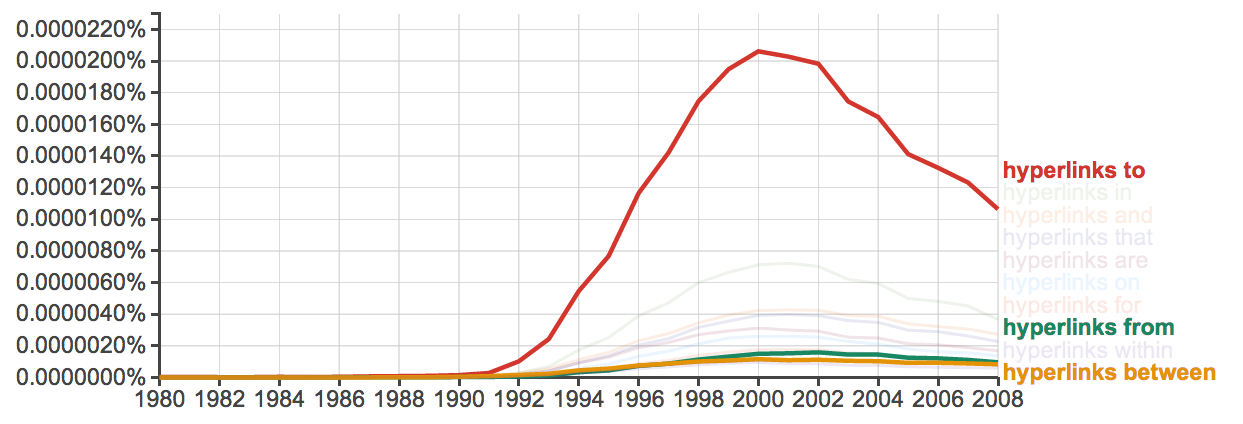
\includegraphics[scale=.25]{chapter6.tex/ngram1}
  }
\caption{Google Ngram Viewer (hyperlinks *)}
\label{ngram-plural}
\end{figure}



\begin{figure}
\centerline{
  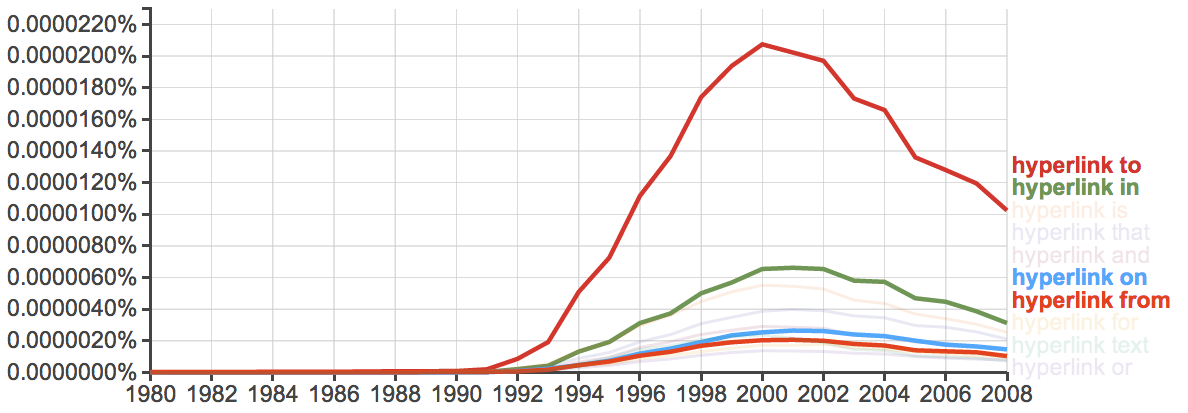
\includegraphics[scale=.25]{chapter6.tex/ngram2}
  }
\caption{Google Ngram Viewer (hyperlink *)}
\label{ngram-singular}
\end{figure}
\begin{sloppier}
In some sense, we are wired to understand the world this way.  Our conceptual system has properties grounded in perception --- both physically and socially \citep{Lakoff:2008tq}. Thought and reason are not simply linguistic abstractions but come from an intimate understanding the physical world around us.
\end{sloppier}


\subsection{Usability of Hyperlinked Icons}
\label{usabilityofhyperlinkedicons}

There appears to be little relevant research (if any) on the topic of hyperlinked images. However, there exists some on the topic of icons.  \citet*{Cheng:2007eh}  studied the use of iconic hyperlinks on e-commerce websites. Not surprisingly, they found that easily identifiable icons increase system usability. Those that are ambiguous affect the rate of task performance.  \citet*{Wiedenbeck:1999vk}  specifically examined the effect of combining text labels with icons. For a learning-based task, performance was poorest on icon-only interfaces, however, once learned, perception of ease of use was higher.

The pre-pilot discussed in the next section explores how people understand indexicality in the context of advertisements.

\section{Pre-Pilot}
\label{pre-pilot}

The purpose of this pre-pilot was to better understand how users perceive and interact with advertisements composed of graphical and iconic elements. 

\subsection{Method and Procedure}
\label{methodandprocedure}

Between the dates of 7--14 October 2013, I created an AMT assignment for 10 workers to annotate a series of approximately 25 images. For this task, I paid \$0.75. 

There were two groups of images representing two tasks. The first four image annotations were a test to see whether there might be a tangible effect of a ``call-to-action'' button icon on an ad. That is, would the presence of an iconic button influence where a person clicked on an ad. For these images, participants were given a screen shot of a digital news article and asked ``Please find the [Ford] Ad and click on it'' (substituting the brand name as appropriate).

The 21 remaining images comprised the second task which explored participant perception of image advertisements, including those containing the AdChoices icon. Workers were presented ads in isolation and asked to click on ``clickable things''. 

Before the second set of images was presented, I provided a short training session to familiarize annotators with the task. 

For the first training task  (\autoref{training-1}),  annotators were asked simply to click on the ad. By clicking, a tiny sticky note was left behind to remind the annotator where they clicked. Annotators were also asked to count the number of clickable things (things that do something or take you somewhere). For the first image, annotators were instructed to select ``1''.


\begin{figure}
\centerline{
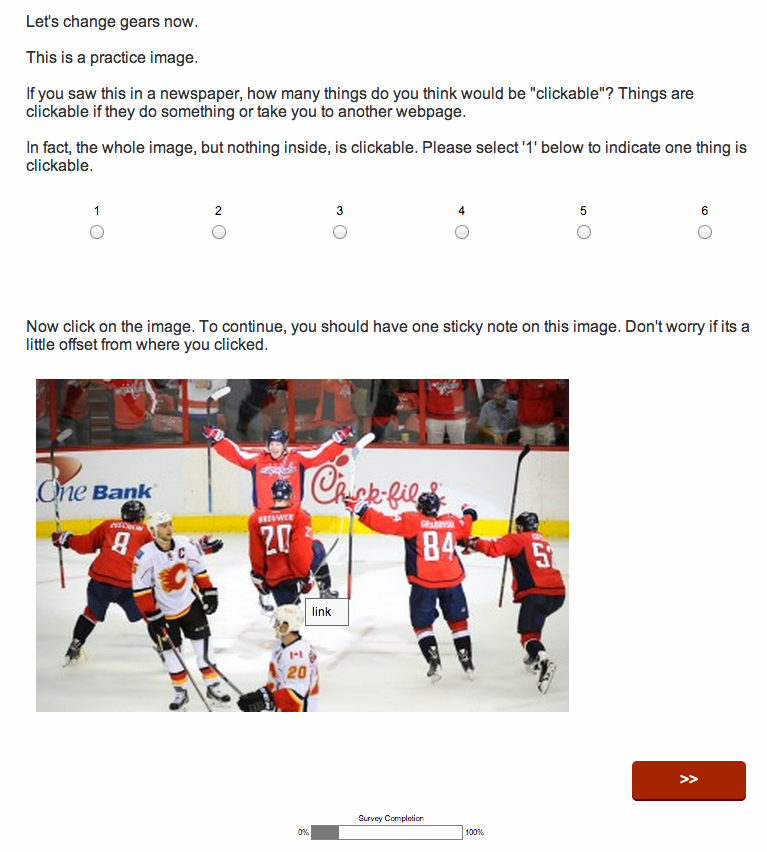
\includegraphics[scale=.3]{chapter6.tex/training1}
}
\caption{Training Task 1}
\label{training-1}
\end{figure}


For the second training task, a typical sign-in \slash  registration box was presented. Participants were instructed that text links and buttons from forms were clickable, but that text entry fields were not  (\autoref{training-2}). 


\begin{figure}
\centerline{
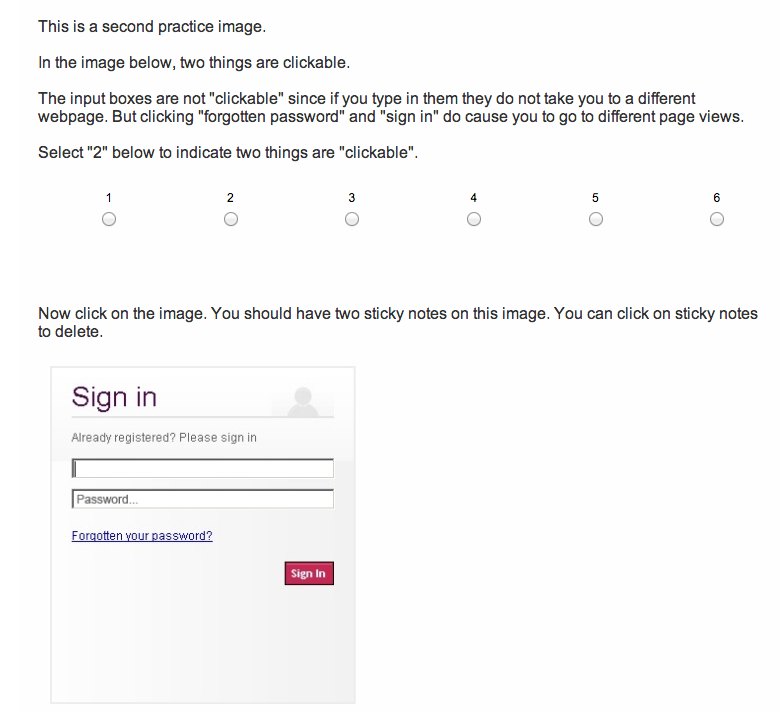
\includegraphics[scale=.3]{chapter6.tex/training2}
}
\caption{Training Task 2}
\label{training-2}
\end{figure}


Finally, in the third training task, participants were told that there were multiple things one could click on, but there were only three links  (\autoref{training-3}). 

\begin{figure}
\centerline{
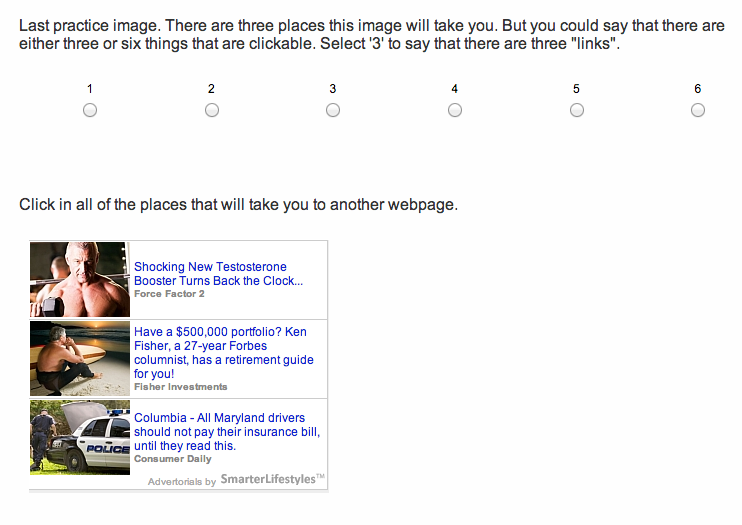
\includegraphics[scale=.3]{chapter6.tex/training3}
}
\caption{Training Task 3}
\label{training-3}
\end{figure}


After annotators completed all three training tasks, they were presented images to annotate on their own. A typical image annotation task is shown in  \autoref{prepilot-task}. 


\begin{figure}
\centerline{
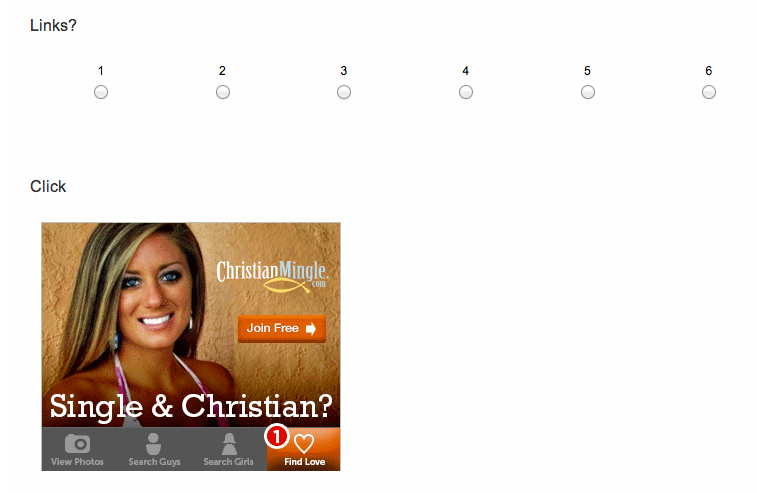
\includegraphics[scale=.3]{chapter6.tex/example1}
}
\caption{Image Annotation Task}
\label{prepilot-task}
\end{figure}


\subsection{Results and Discussion}
\label{resultsanddiscussion}

Results from the first four heat map visualizations appear in  \autoref{prepilot-ford}, \autoref{prepilot-cars}, \autoref{prepilot-travelers}, \autoref{prepilot-visa}. 


\begin{figure}
\centerline{
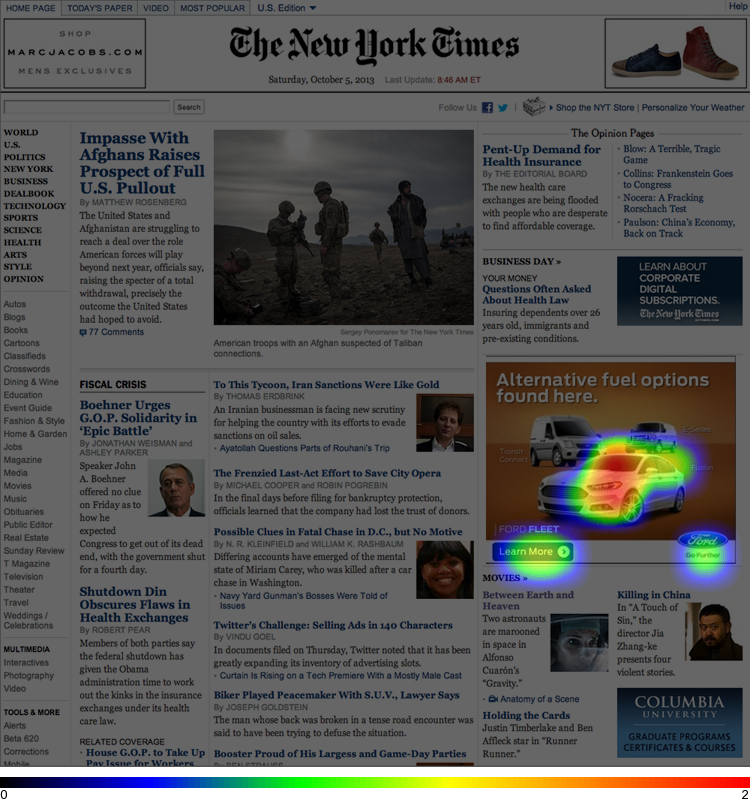
\includegraphics[scale=.3]{chapter6.tex/ford-hotspot}
}
\caption{Ford Ad}
\label{prepilot-ford}
\end{figure}

\begin{figure}
\centerline{
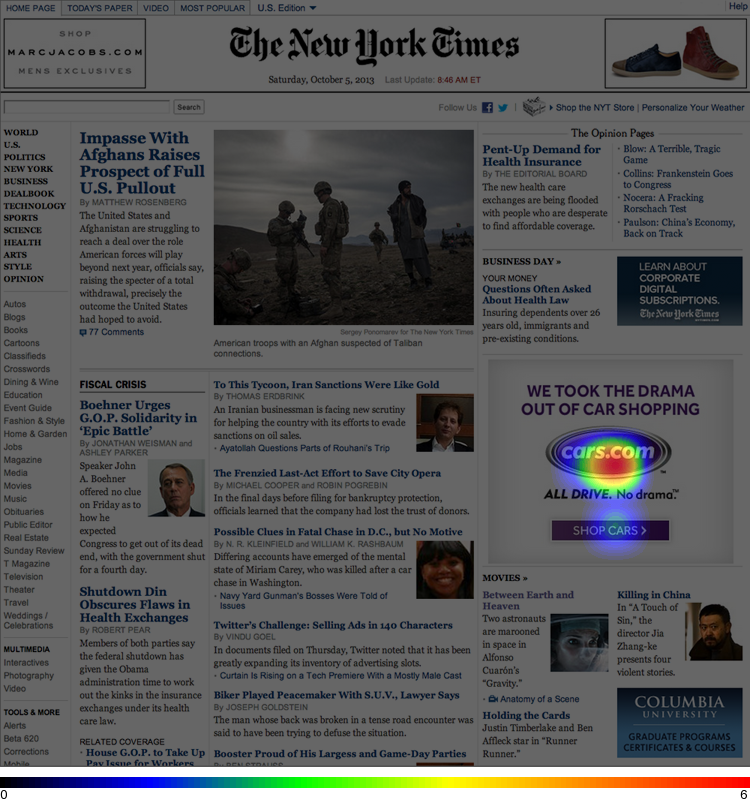
\includegraphics[scale=.3]{chapter6.tex/cars-hotspot}
}
\caption{Cars.com Ad}
\label{prepilot-cars}
\end{figure}

\begin{figure}
\centerline{
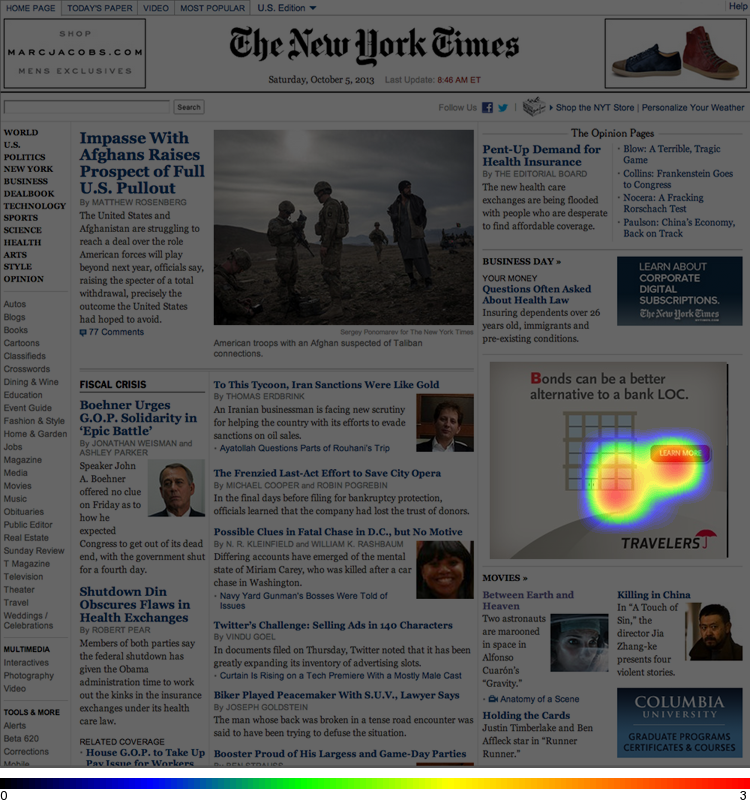
\includegraphics[scale=.3]{chapter6.tex/travelers-hotspot}
}
\caption{Traveler's Ad}
\label{prepilot-travelers}
\end{figure}

\begin{figure}
\centerline{
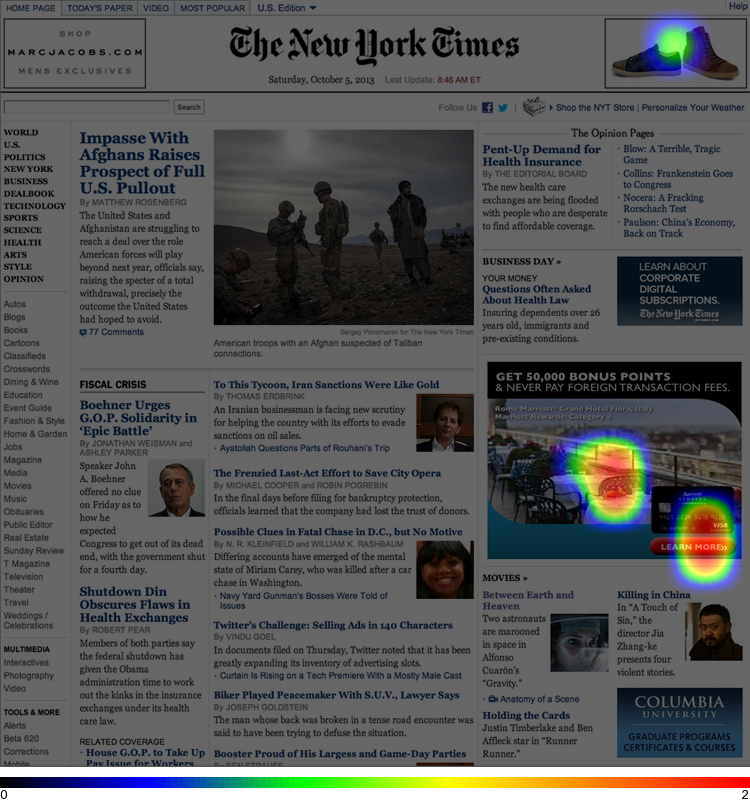
\includegraphics[scale=.3]{chapter6.tex/visa-hotspot}
}
\caption{Visa Ad}
\label{prepilot-visa}
\end{figure}

In each of the four images, one or more participants clicked directly on the iconic button link, despite implicit knowledge that the ad itself was hyperlinked to the advertiser's landing page. In addition, it appears that brands iconic in shape and style as buttons, also elicited clicks. Note the distinctive shape of the Ford logo in the first image and cars.com logo in the second. However, it could also be said that most clicked on the center of an ad, rather than on a button or iconic brand image.

 \autoref{complex-result}  shows the result for the example task 2 image above:

\begin{figure}
\centerline{
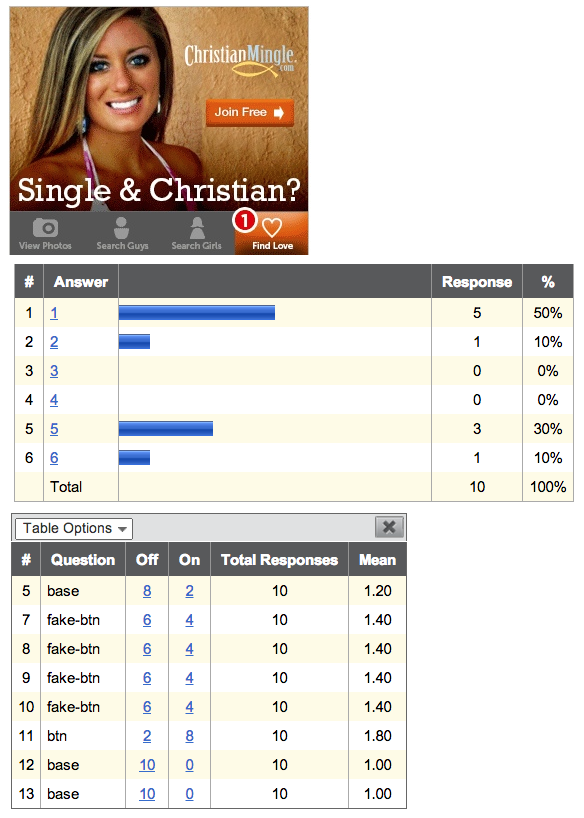
\includegraphics[scale=.3]{chapter6.tex/example1-annotated}
}
\caption{Results for Complex Ad}
\label{complex-result}
\end{figure}

Roughly half of the participants saw this ad as containing only one link. Others appeared to see fake buttons as links.

 \autoref{prepilot-twitter}  is another example from task 2. Here you can see that half of the annotators clicked on the Twitter icon.

\begin{figure}
\centerline{
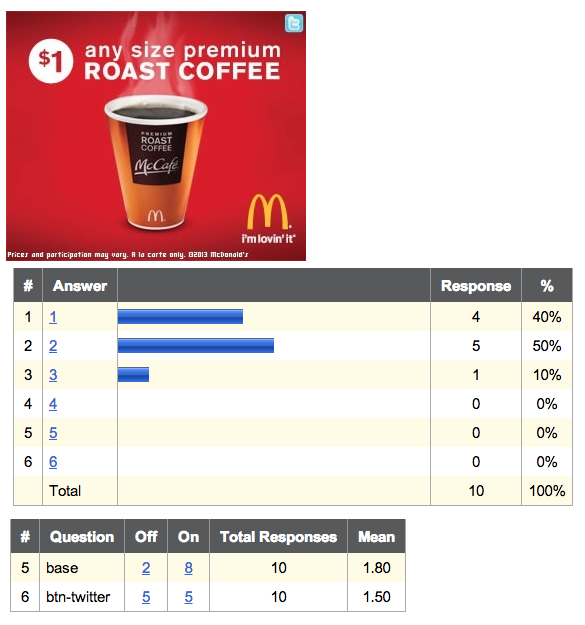
\includegraphics[scale=.5]{chapter6.tex/twitter-example}
}
\caption{Results for McDonald's Ad with Twitter Icon}
\label{prepilot-twitter}
\end{figure}



\begin{figure}
\centerline{
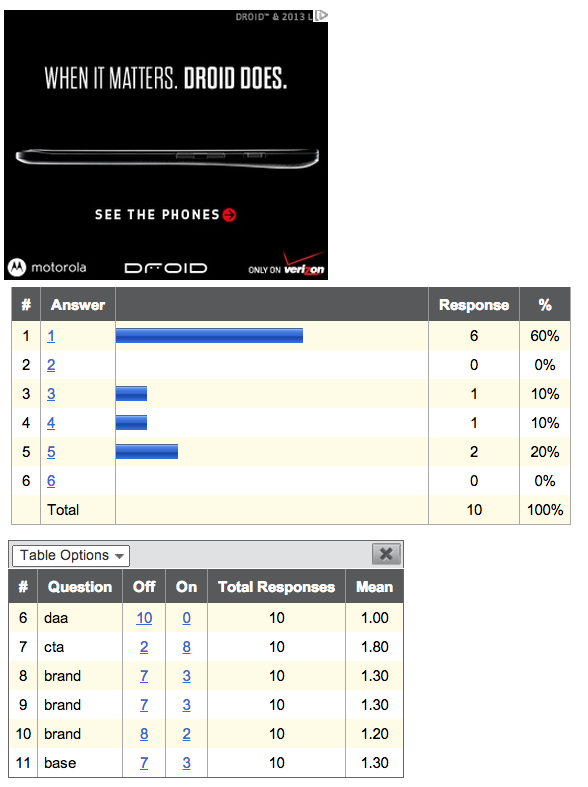
\includegraphics[scale=.3]{chapter6.tex/daa-example}
}
\caption{Android Ad with AdChoices Icon}
\label{prepilot-adchoices}
\end{figure}


Finally,  \autoref{prepilot-adchoices}  is an ad with the AdChoices icon. No one clicked on the AdChoices icon. But 8 of 10 clicked on the ``See the Phones'' call-to-action. And several each clicked on the Motorola, Droid, and Verizon brands at the bottom of the image.

By examining task 2 results, I learned that my task was too complex and it was possible participants may have mis-understood what was asked of them. However, the pre-pilot also proved the feasibility of studying user perception of the indexicality of advertisements. This simple qualitative study provided insight valuable to the design and implementation of controlled experiments.

\section{Aims}
\label{aims}

In this pilot, I consider indexical reference in hyperlinked advertisements in the context of task-based interaction. In experiment 2A I look at how knowledge contributes to perception of an indexical link on a brand icon. In experiment 2B, I look at iconic buttons on advertisements to see if the presence of a button affects where a user clicks on an ad.

\section{Experimental Design}
\label{experimentaldesign}

Study 1A considers the proposition that iconic elements of advertisements are perceived as indexical if people know what the icon represents, it contrasts semantically with the advertisement, and it signals communicative intent (for example, as a ``call-to-action''). This breaks down into to three study different hypotheses.

\begin{description}
\item{Hypothesis 2A1} \hfill \\ 
Known icons, embedded in advertisements, with brands contrastive to the background advertisement, are perceived differently than icons that semantically match the brand of the primary advertisement.
\end{description}
A McDonald's icon on a McDonald's ad should not be seen as indexical: merely iconic. However, an Apple icon on a McDonald's site might be considered indexical.
\begin{description}
\item{Hypothesis 2A2} \hfill \\
Known icons, embedded in advertisements, are perceived differently than those that are unknown.
\end{description}
This hypothesis predicts that icons which are unknown may be treated differently than those that are known. That is, a fake brand may be perceived differently than the known Apple brand. Likewise, the AdChoices icon, if unknown, should be treated as an unknown brand.
\begin{description}
\item{Hypothesis 2A3} \hfill \\
An icon that signals action is perceived differently than an icon that does not signal action.
\end{description}

A Twitter logo (as appears in \autoref{social-media}) is iconic and known to serve one of several functions: "tweet" or "go to Twitter" (to tweet/follow). Likewise, a plain FaceBook icon (also in \autoref{social-media} may be perceived to function as "share" or "go to FaceBook" (to share/follow).\footnote{These observations are made on the basis of a short AMT survey where I asked 40 turkers what they thought these icons meant in the context of the Yahoo news article in \autoref{social-media}.} That people know these things about Twitter and FaceBook is a function of their relative popularity online.  Hypothesis 2A3 predicts that icons, known or unknown, will be perceived differently if they signal action such as share/follow/post/goto, etc.

\begin{figure}
\centerline{
  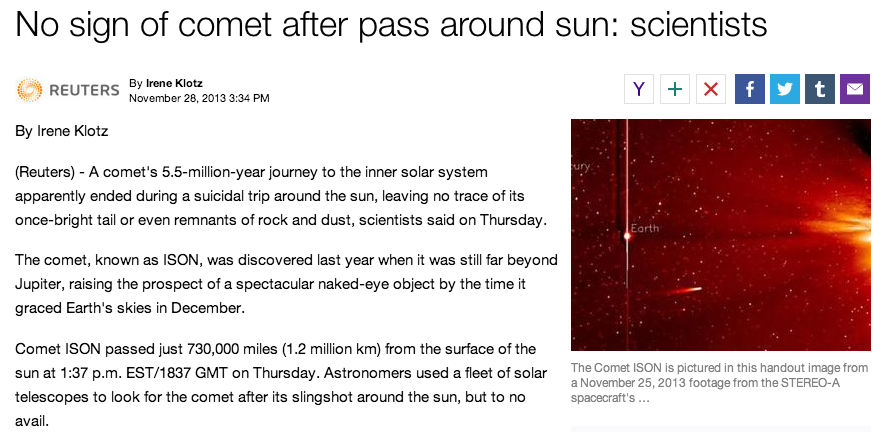
\includegraphics[scale=.3]{chapter6.tex/socialmedia}
  }
\caption{Twitter and FaceBook Icons}
\label{social-media}
\end{figure}


Experiment 2A is a single factor posttest-only design. There is one \textbf{independent variable with 5 levels}: ``same brand'', ``different brand'', ``unknown brand'', ``known signal'', and ``AdChoices''. There is one \textbf{dependent variable}: perception of an indexical reference. Five groups are required. The control group sees a McDonald's ad with an icon McDonald's logo in the upper right hand corner. Other groups see a different logo of the same size in the same place: Apple, Unknown, FaceBook, and AdChoices. Apple and FaceBook logos were chosen since they have among the highest global brand recognition  \citep{Interbrand:aa}. 
 
\begin{description}
\item{Hypothesis 2B} \hfill \\
Iconic graphical elements influence the click behavior by affecting where people click.
\end{description}

Experiment 2B is a single factor posttest-only design with three levels. The control and two treatment groups are presented with a a newspaper article containing an ad. The control group receives an ad with no ``call-to-action'', while one treatment group sees the same ad but with a textual ``call-to-action'', and the other treatment group sees the same ad with an iconic button containing the same ``call-to-action'' text as the first treatment group. The \textbf{independent variable} is ``icon'' and \textbf{dependent variable} is click location (on the ``call-to-action'' or elsewhere). 

Data for Experiment 2A and 2B were collected in separate events. Following presentation of a single task, survey data was collected.

\section{Method}
\label{method}

These two experimental designs follow the general procedure outlined in Chapter Four.

\subsection{Experiment 2A Method}
\label{experiment2amethod}

\subsubsection{Settings and Participants}
\label{settingsandparticipants}

Using Amazon's Mechanical Turk, 303 workers were paid \$0.15 to participate in one of two conditions of the single-factor design previously described. Participants were assigned randomly via Qualtrics block randomizer. Results were collected during the period of 7--14 October 2014. The task was expected to take approximately three minutes, though workers were allowed up to 10 minutes to complete.

\subsubsection{Procedure and Materials}
\label{procedureandmaterials}


The general procedure follows that described in Chapter Four. \autoref{2A-flow} gives a more detailed graphical depiction of flow.

\begin{figure}
\centerline{
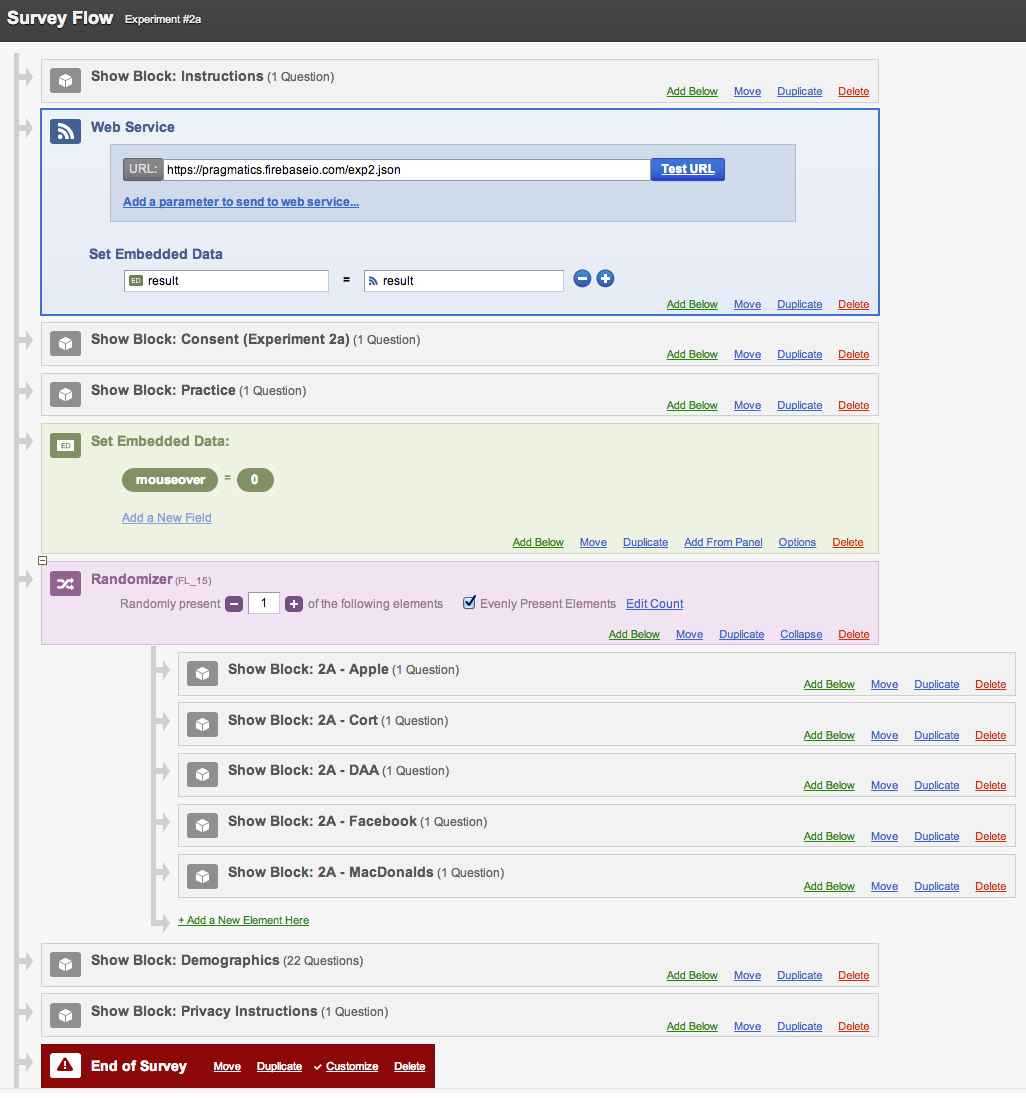
\includegraphics[scale=.3]{chapter6.tex/2a-flow}
}
\caption{Experiment 2A Flow}
\label{2A-flow}
\end{figure}


Following presentation of instructions and consent form, participants were each presented one question, as illustrated in the exemplar in  \autoref{2A-adchoices},  followed by survey questions. Participants were instructed to ``Please click on things you think are links.'' 

The image used was taken from on online article at  \url{http://yahoo.com},  while the advertisement from  \url{http://moat.com}.  Alterations were accomplished using PhotoShop to create five variants. Logos were restricted to a size of approximately 20px x18px to approximate the 19px x15px (icon only with container) size specified by  \cite{Anonymous:2011ur}.  However, all logos including the AdChoices icon were presented with 100\% opacity on a white background, except for the Apple logo which was unaltered as white on a black background.


\begin{figure}
\centerline{
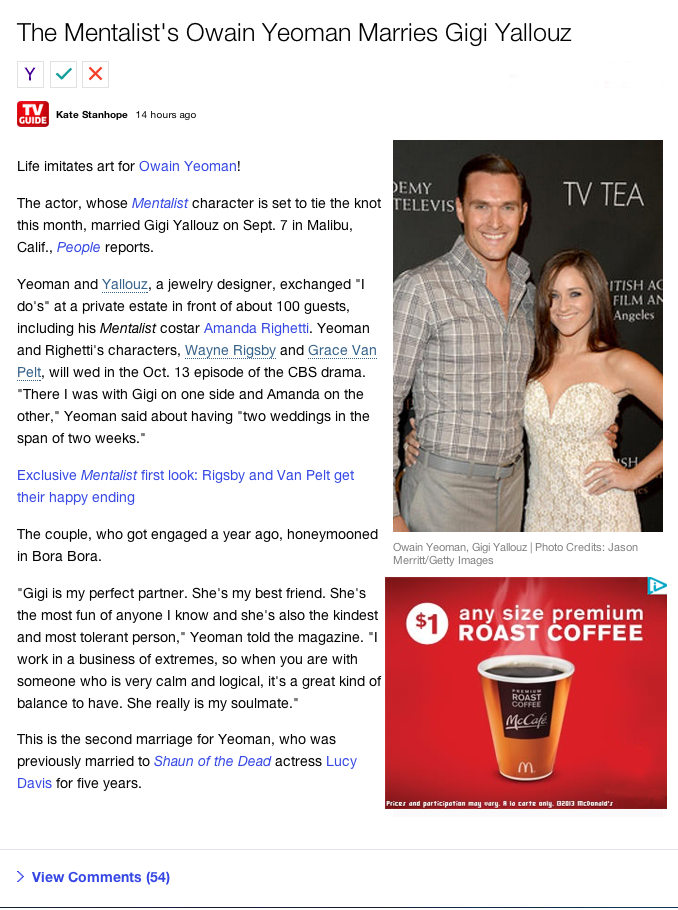
\includegraphics[scale=.3]{chapter6.tex/2a-daa}
}
\caption{McDonald's Ad with AdChoices Icon}
\label{2A-adchoices}
\end{figure}


\subsubsection{Instrumentation}
\label{instrumentation}

In addition to features provided by AMT and Qualtrics, my scripts performed the following:

\begin{sloppier}
\begin{enumerate}
\item Disable preview using a custom CSS class blocking Qualtrics controls
\item Check worker hash against a FireBase web service and request worker to return HIT if the hash is in the exclusion list
\item Add worker hash to FireBase
\item Submit results to AMT on completion of the Qualtrics survey
\item Hide Qualtrics hotspot regions from mouseovers
\item  Create "sticky" notes on clicks
\item  Observe whether mouseovers were detected over treatment icons
\end{enumerate}
\end{sloppier}

The last three capabilities were developed as custom code for this particular experiment. Qualtrics provides two image annotation capabilities, both of which are limited in some respect. 

The heat map annotation provided by Qualtrics used in the pre-pilot, required that the number of clicks be pre-specified by the experimenter. This is not desirable for tasks in which participants will click an arbitrary number of times. 

Instead, I used the hotspot annotation capability provided by Qualtrics. This let me create image zones to detect where a user clicks. Unfortunately, Qualtrics zones become visible when a participant mouses over a region. For the purposes of the pre-pilot and Experiment 2, I modified the Qualtrics hotspot capability in two ways: 1) never show zones; and 2) clicking creates a small sticky note so that the participant can see some evidence of click feedback at the location of the click.

\subsection{Experiment 2B Method}
\label{experiment2bmethod}

\subsubsection{Settings and Participants}
\label{settingsandparticipants}

Using Amazon's Mechanical Turk, 202 workers were paid \$0.15 to participate in one of two conditions of the single factor design previously described. Participants were assigned randomly via Qualtrics block randomizer. Results were collected between the days of 7--14 October 2013. The task was expected to take approximately three minutes, though workers were allowed up to 10 minutes to complete.

\subsubsection{Procedure and Materials}
\label{procedureandmaterials}

The general procedure follows that described in Chapter Four.  \autoref{1B-flow}  gives a more detailed graphical depiction of flow.

\begin{figure}
\centerline{
  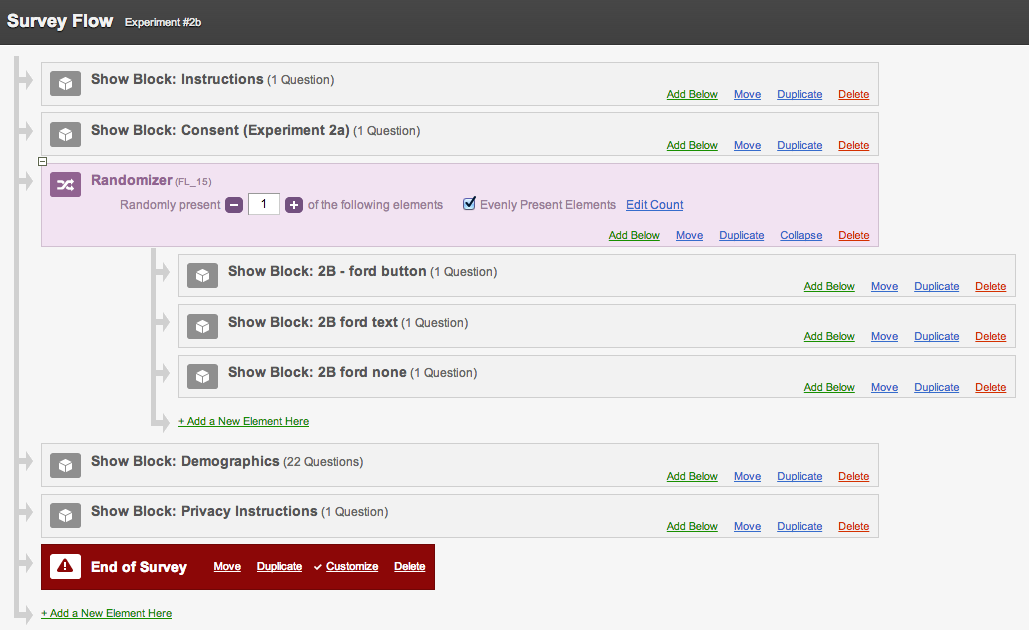
\includegraphics[scale=.3]{chapter6.tex/2b-flow}
  }
\caption{Experiment 2B Flow}
\label{1B-flow}
\end{figure}

Following presentation of instructions and consent form, participants were presented a screen shot from a \emph{The New York Times} article with my ad substituting for the same-sized block ad in which an ad originally appeared. I used the Ford ad that had been previously used in the pre-pilot  (same as figure \autoref{prepilot-ford}).  Participants were instructed, ``pretend you are interested in getting a hybrid car. Find the Ford ad and click on it.''

\subsubsection{Instrumentation}
\label{instrumentation}

In addition to features provided by AMT and Qualtrics, my scripts performed the following:

\begin{sloppier}
\begin{enumerate}
\item Disable preview using a custom CSS class blocking Qualtrics controls
\item Add worker hash to FireBase
\item Submit results to AMT on completion of the Qualtrics survey
\end{enumerate}
\end{sloppier}

In this experiment, I used the heat map capability of Qualtrics since only one click was requested.

\section{Data Collected}
\label{datacollected}

Using G* Power 3  \citep{PowerAnalysisIntro:2012uy}  chi square goodness of fit test, for both experiments I estimated a sample size of approximately 220 was necessary in order to detect a medium effect with power of 0.95. All surveys initiated were completed: there were no known drop-outs.

Once all assignments had been completed, (as indicated on my AMT requester dashboard), I downloaded data as a single CSV (comma separated values) file from the Qualtrics website. Data was organized such that each participant's data was on its own row.

\section{Results}
\label{results}

\subsection{Experiment 2A Results}
\label{experiment2aresults}

Because the IV is categorical (binary), a non-parametric statistics is required. Strikingly, there are very few clicks on icons at all.


\begin{table}
\caption{2A Raw Clicks}
\centering
\begin{tabular}{ccc}
Clicks & Total & Icon\tabularnewline
1 & 60 & Apple\tabularnewline
2 & 59 & Unknown\tabularnewline
2 & 58 & AdChoices\tabularnewline
10 & 52 & FaceBook\tabularnewline
0 & 59 & MacDonald's\tabularnewline
\end{tabular}
\end{table}


9\% (27 of 303) of participants said they recognized the AdChoices icon, though when questioned what it meant, only 5.6\% were correct. Of the two that clicked on the AdChoices icon, one was correct and the other mistakenly believed it would link to the advertiser's page. Of 303 participants, there were 21 mouseover events over icons --- 3 (including the two that clicked) over the AdChoices icon. This means, that had the AdChoices icon been animated on mouseover, one additional person might have been alerted that the icon was meaningful.

Given relatively little data, it is difficult to come to any strong conclusion. Results suggest that the effect size was considerably smaller than anticipated. In the pre-pilot, approximately 50\% (5 of 10) clicked the Twitter icon. In this study, only 19\% of those presented with the FaceBook icon clicked on it. As a follow-up, I added a condition that simply enlarged the icon to approximately twice the size (30px x 28px). This had no effect: only 17\% (10\slash 58) presented with the larger FaceBook icon clicked on it.

I also considered that it might be possible that, despite studies showing little difference in quality of annotation with price variation, amount of pay might might be a factor. However, I ran another 200 subjects at a higher pay rate (25 cents for a 2-minute task). This also caused no change.

It is still possible, that the small number of click observations could reflect omission effects of the paid volunteer  \citep{Rush:1978tw}.  This remains un-tested.

Finally, the pre-collection focused on images in isolation.  \graffito{Committee: I will re-run this in isolation over the Holidays. I may also test both Twitter \& FB icons.} This experiment placed ads in context. It is quite possible this accounts for differences seen. Typically, linguistic judgment tasks are presented under isolated conditions where external context plays no role. However, this experiment afforded the opportunity to observe participant behavior under relatively natural conditions and was useful for this reason, if no other.

Though I created additional stimuli, due to time constraints, they were not used in this experiment. As with Experiment 1, advertisements as stimuli (and, indeed, the background newspaper itself) introduce random effects. Thus, the results presented here do not necessarily generalize across all advertisements or embedded contexts. 

\subsection{Experiment 2B Results}
\label{experiment2bresults}

 \autoref{2B-results}  presents raw frequency counts for each of the three conditions. 


\begin{table}
\caption{2B Results}
\label{2B-results}
\centering
\begin{tabular}{cccc}
 & Button & Logo & Other\tabularnewline
\cline{2-4} 
None & 0 & 2 & 64\tabularnewline
Text & 0 & 1 & 66\tabularnewline
Button & 1 & 1 & 67\tabularnewline
\end{tabular}
\end{table}


As before, because the IV is categorical (binary), a non-parametric statistics is required. Again, some cell counts were quite low and, overall, unbalanced --- so I used a Fisher's Exact Test. The p-value was equal to 1 indicating no significant difference between conditions.

As in 2A, results differed somewhat from the pre-pilot. The difference here was the title of task and payment amount, plus slight variation in the instructions. It is possible that the effect size here was simply too small to detect. A\slash B testing of ads generally involve a large number of subjects such that it might be possible to detect actual effects on behavior where none in this size study was seen. 

This task was also presented in the context of a news article and not in isolation, as had been in the pre-pilot.  \graffito{Committee: I will re-run this in isolation over the Holidays.}  As with 2A, I ran a follow-up study offering 25 cents for a shorter task. There was no effect on performance. It is possible that a larger effect size might be observed if the task were presented in isolation, rather than in context.
